\section{Detector Model}
\label{sec:detector_description}
{\bf Copy info from~\cite{Aberle2014}.

Figures~\ref{fig:ArrivalTimeDist} and~\ref{fig:NPhotDist} show simulation
output relevant for further discussion.}

\begin{figure*}[ht]
  \centering
  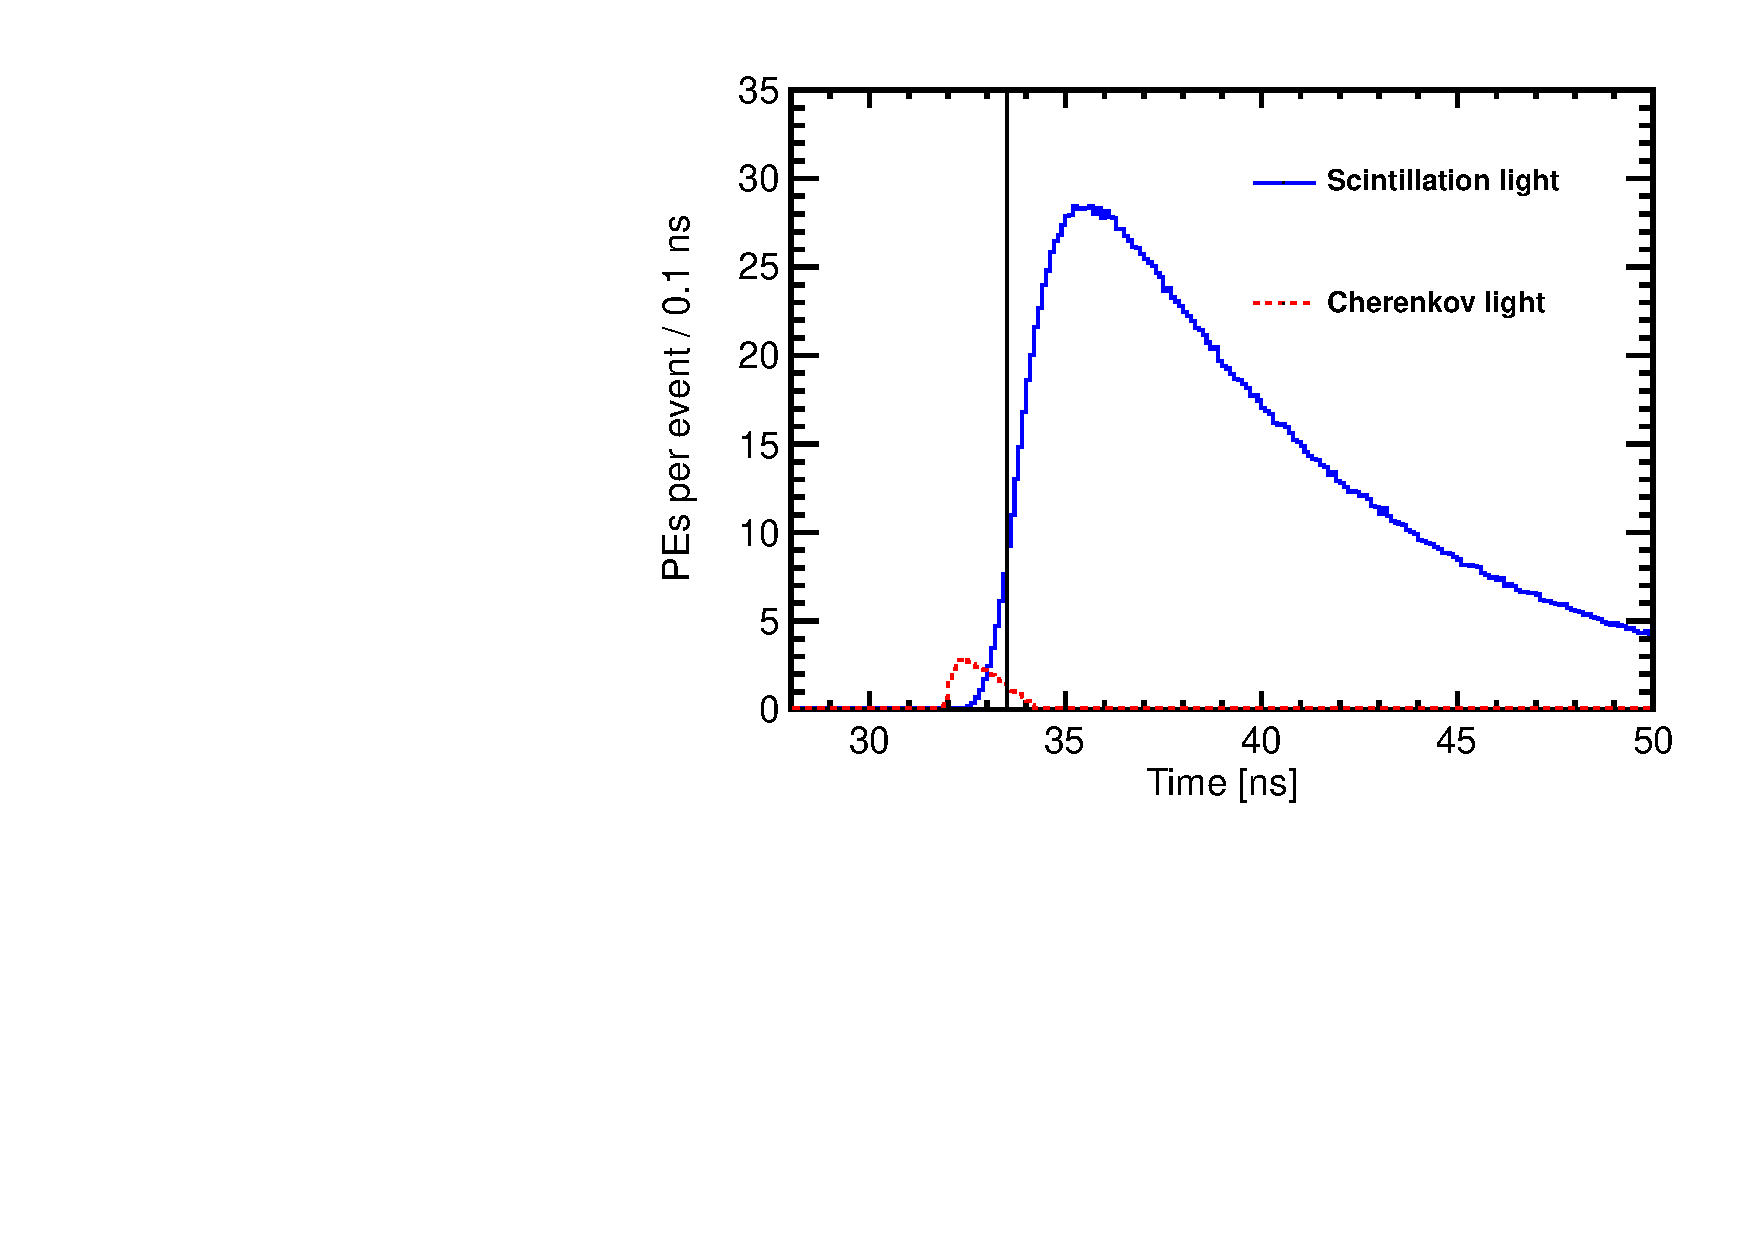
\includegraphics[width=0.45\textwidth]{hT_Te130.pdf}
  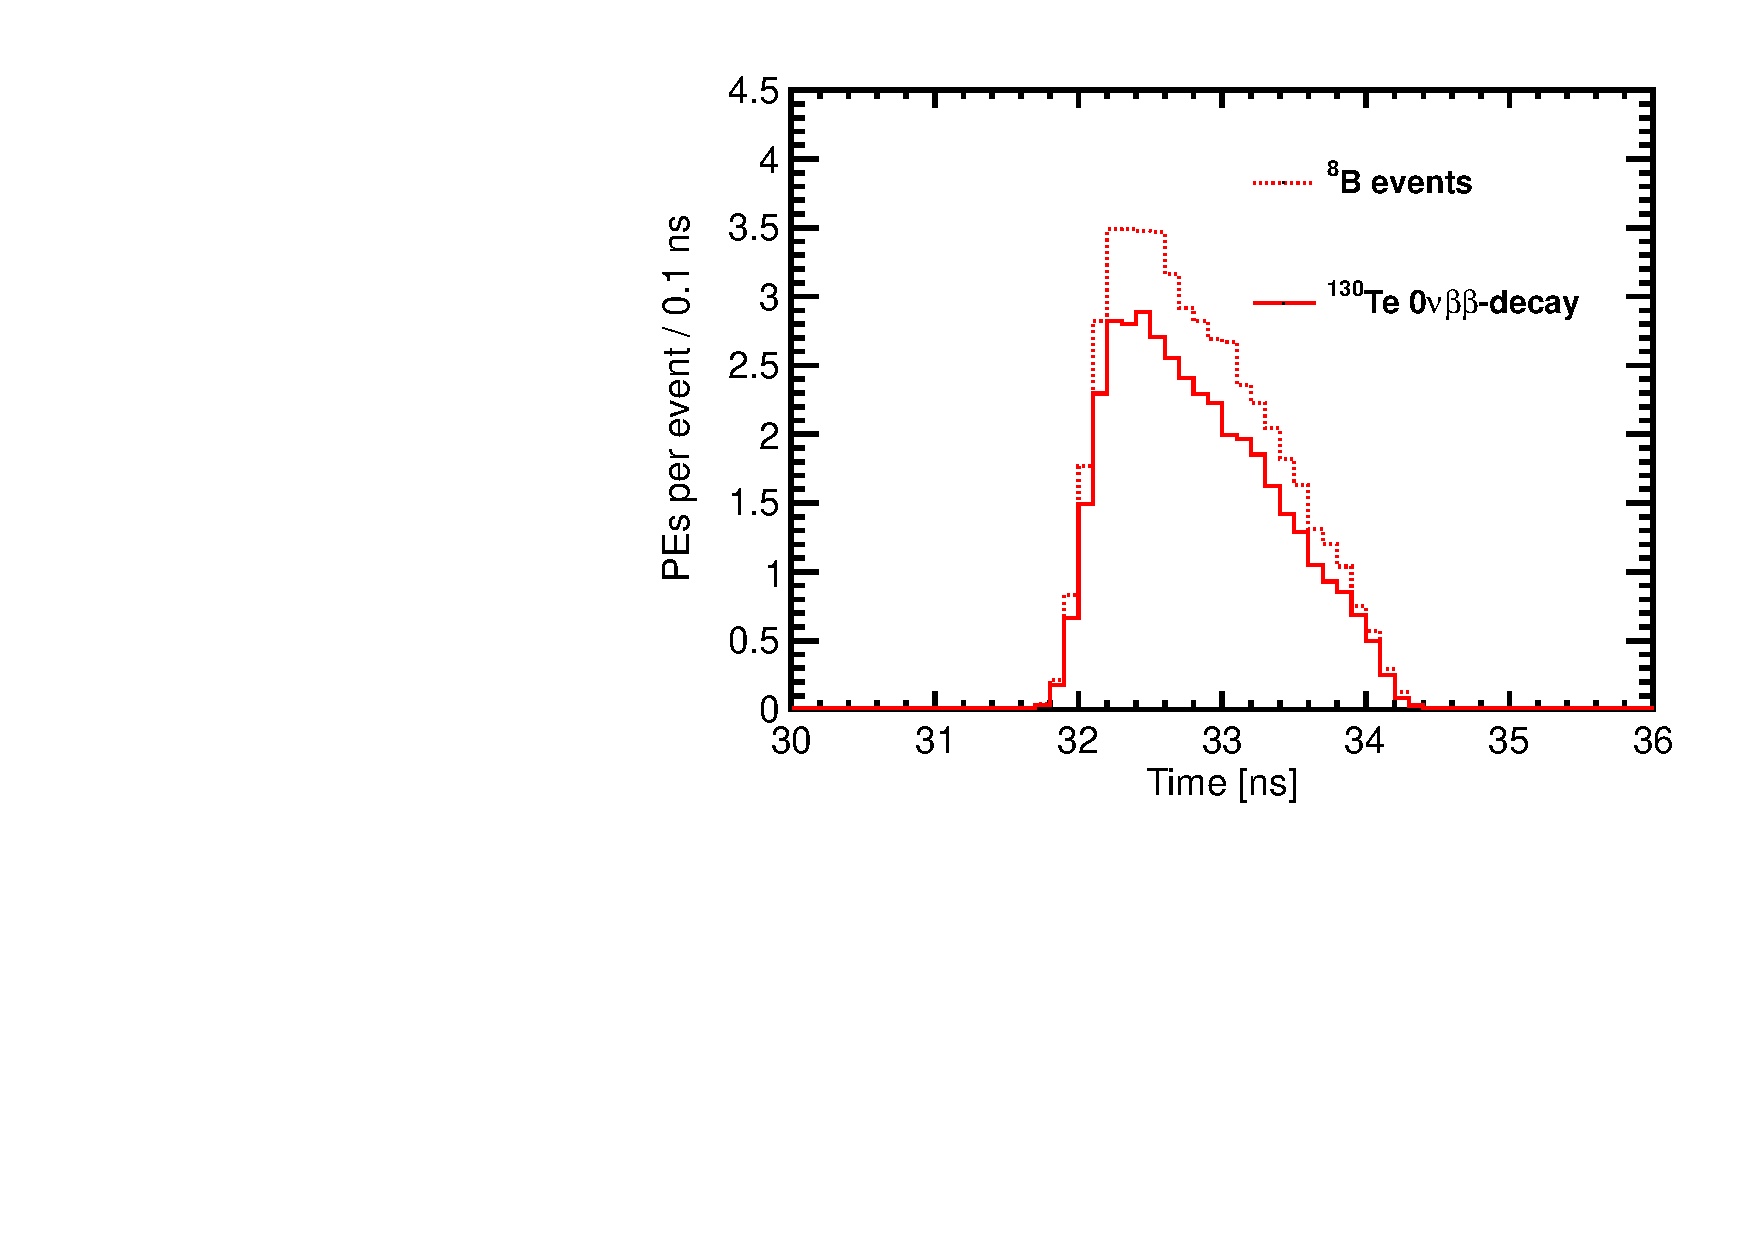
\includegraphics[width=0.45\textwidth]{hTche_Te130_B8.pdf}
  \caption{\emph{Left:} Photo-electron (PE) arrival times after
    application of the photo-detector transit time spread (TTS) of
    100~ps for the simulation of 1000 0{\nbb} decay events of
    $^{130}$Te at the center of the detector. PEs from Cherenkov light
    (\emph{dashed red line}) and scintillation light (\emph{solid blue
      line}) are compared. The black vertical line illustrates a time
    cut at 33.5 ns. \emph{Right:} Comparison between Cherenkov PEs
    arrival time for $^{130}$Te {0\nbb} decay (\emph{solid line}) and
    $^{8}$B (\emph{dotted line}) events. {\bf Distributions of the
      scintillation PEs arrival time are indistinguishable between
      $^{130}$Te 0{\nbb} decay and $^8$B due to identical total energy
      in the event, $Q(^{130}{\rm Te})=2.526$~MeV.} }
\label{fig:ArrivalTimeDist}
\end{figure*}


\begin{figure*}[ht]
  \centering
  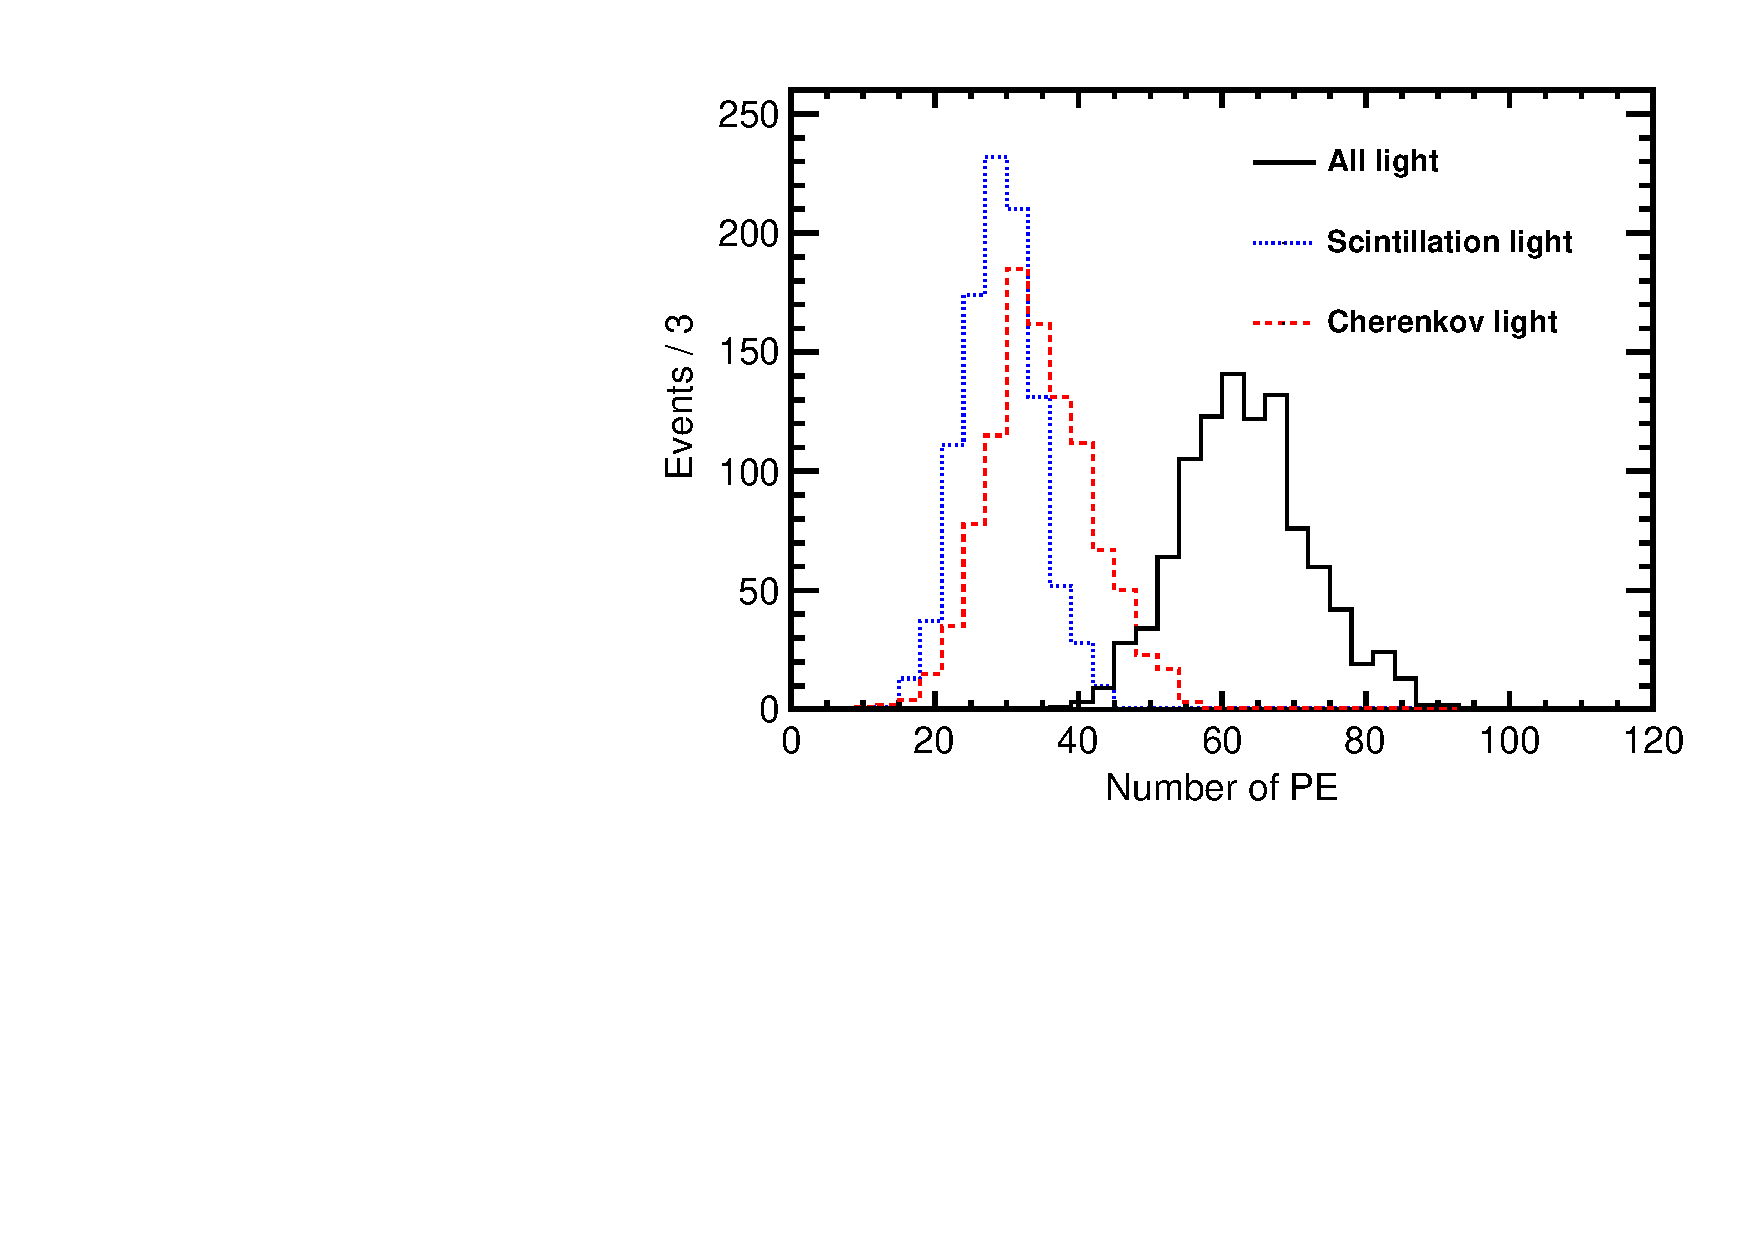
\includegraphics[width=0.45\textwidth]{hMomNPhot_Te130.pdf}
  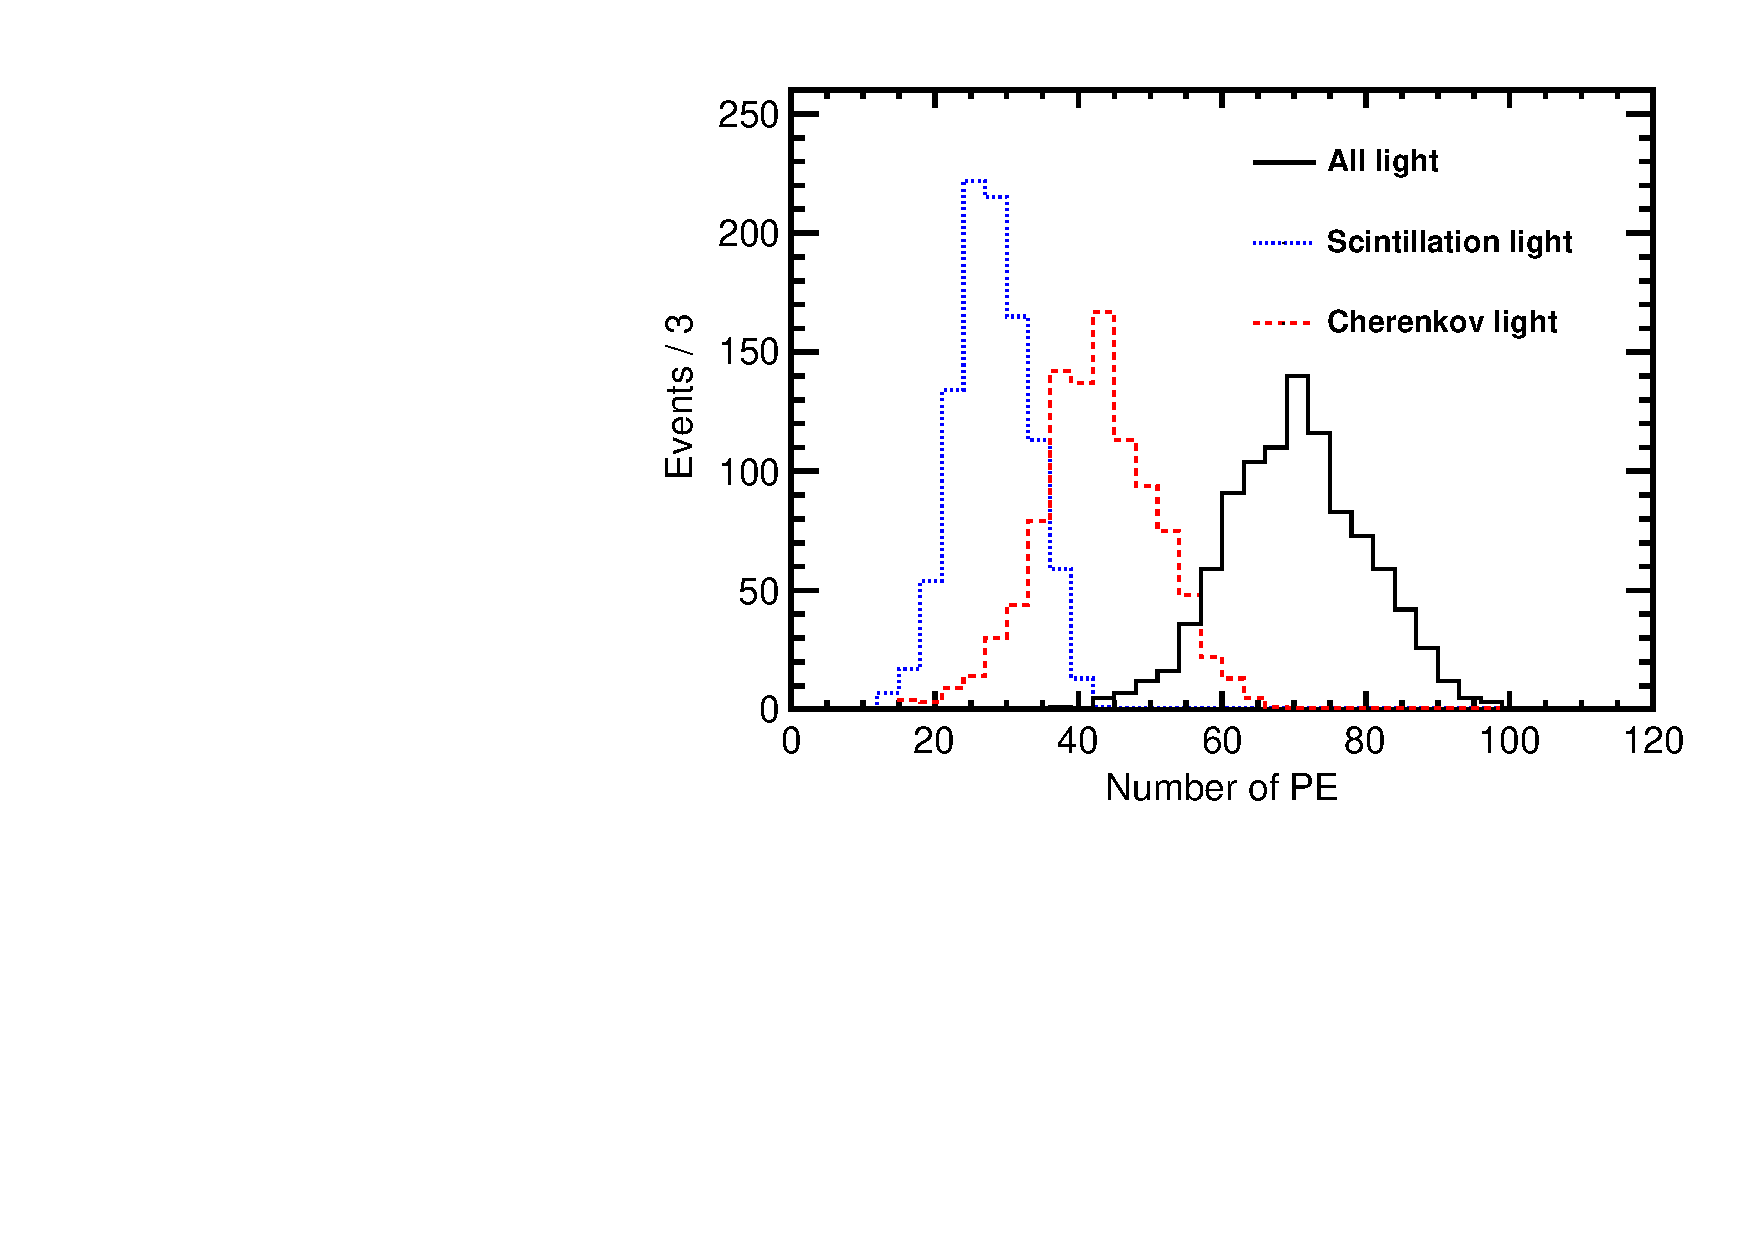
\includegraphics[width=0.45\textwidth]{hMomNPhot_1el_2p529MeV.pdf}
  \caption{Number of Cherenkov (\emph{dashed red line}), scintillation
    (\emph{dotted blue line}), and total (\emph{solid black line}) PEs
    for the simulation of 1000 $^{130}$Te 0{\nbb} decay (left panel)
    and $^8$B (\emph{right panel}) events.}
\label{fig:NPhotDist}
\end{figure*}

